\documentclass[english,bachelor,a4paper,oneside,draft,12pt]{ppfcmthesis}

\usepackage[utf8]{inputenc}

\usepackage[T1]{fontenc}
\usepackage[urw-garamond]{mathdesign}

\usepackage{amsfonts}
\usepackage{amsmath}

\usepackage{algorithm}
\usepackage[noend]{algorithmicplus}
\usepackage{listings}

\renewcommand{\tt}{\ttfamily}
\newcommand{\code}[1]{{\ttfamily #1}}
\newcommand{\PYG}[2]{#2}

\newcounter{tightListCounter}

% no extra spacing between lines
\newenvironment{tightList}[1][]
{
  \begin{list}{
                  \arabic{tightListCounter}.
              }
              {
                  \usecounter{tightListCounter}
                  \setlength{\topsep}{0.0em}
                  \setlength{\itemsep}{0.0em}
                  \setlength{\parsep}{0.0em}
                  \setlength{\listparindent}{0.0em}
                  #1
              }
}
{
  \end{list}
}

% Authors here.
\author{%
   Jan Kończak \album{84822} \and 
   Tomasz Żurkowski \album{84915}}
\authortitle{}                                        % Do not change.
 \title{{\Huge JPaxos} \hspace{5em} State~machine~replication based~on~the~Paxos~protocol}
%\title{JPaxos State~machine~replication based~on~the~Paxos~protocol}
 \titleNoFormat{JPaxos. State~machine~replication based~on~the~Paxos~protocol}
\ppsupervisor{dr hab. inż. Paweł T. Wojciechowski} % Your supervisor comes here.
\ppyear{2011}                                         % Year of final submission (not graduation!)


% commands here
\newenvironment{TODO}
{\begin{center}\par\noindent
{\huge \vspace{-3em} \par\noindent  \rule{0.85\textwidth}{0.1em}  \\ \vspace{-1em} \nointerlineskip
    \[ \mathbf{T} \, _\mathcal{O} \:\: \mathfrak{D} \, _\mathbb{O} \] }
    \begin{minipage}{0.8\textwidth}
}{\end{minipage} {\huge \vspace{-0.5em} \rule{0.85\textwidth}{0.1em}} \par\noindent \end{center} \par}

% Custom commands
\newcommand{\paragraphNewline}[1]
{
  %\paragraph{#1} \hfill
  \paragraph{#1}
  \par \noindent \par \noindent \ignorespaces
}
\newcommand{\paxosJava}[1][ ]{\textsc{PaxosJava#1}}
\newcommand{\alive}[1][ ]{\textsc{Alive#1}}
\newcommand{\prepare}[1][ ]{\textsc{Prepare#1}}
\newcommand{\prepareOK}[1][ ]{\textsc{PrepareOK#1}}
\newcommand{\propose}[1][ ]{\textsc{Propose#1}}
\newcommand{\accept}[1][ ]{\textsc{Accept#1}}
\newcommand{\catchUpQuery}[1][ ]{\textsc{Catch\-Up\-Query#1}}
\newcommand{\catchUpResponse}[1][ ]{\textsc{Catch\-Up\-Response#1}}
\newcommand{\catchUpSnapshot}[1][ ]{\textsc{CatchUpSnapshot#1}}
\newcommand{\proposer}[1][ ]{\textsc{Proposer#1}}
\newcommand{\acceptor}[1][ ]{\textsc{Acceptor#1}}
\newcommand{\learner}[1][ ]{\textsc{Learner#1}}
\newcommand{\recovery}[1][ ]{\textsc{Recovery#1}}
\newcommand{\recoveryAnswer}[1][ ]{\textsc{RecoveryAnswer#1}}


% From Nuno
\newconstruct{\INIT}{\textbf{Initialization:}}{}{\ENDINIT}{}
\newconstruct{\EVERY}{\textbf{every}}{}{\ENDEVERY}{}
\newconstruct{\UPON}{\textbf{upon}}{}{\ENDUPON}{\textbf{end upon}}
\newconstruct{\PROCEDURE}{\textbf{procedure}}{}{\ENDPROC}{\textbf{end procedure}}
\newcommand\BLANK{\SPACE}
\renewcommand{\mod}{\mathrm{~mod~}}


\usepackage{hyperref}
\hypersetup{% Set pdf properties
pdftitle = {JPaxos. State machine replication based on the Paxos protocol},%
pdfauthor = {Jan Kończak, Tomasz Żurkowski},%
pdfsubject = {JPaxos},%
pdfkeywords = {paxos} {state machine} {replication} {consensus} {recovery}%
 {atomic broadcast} {group communication} {reliable services},%
}

\begin{document}

% Front matter starts here
\frontmatter\pagestyle{empty}%
\maketitle\cleardoublepage%

% Blank info page for "karta dyplomowa"
\thispagestyle{empty}\vspace*{\fill}%
\begin{center}Tutaj przychodzi karta pracy dyplomowej;\\oryginał wstawiamy do wersji dla archiwum PP, w pozostałych kopiach wstawiamy ksero.\end{center}%
\vfill\cleardoublepage%

% abstract is already on ``karta dyplomowa''

% Table of contents.
\pagenumbering{Roman}\pagestyle{ppfcmthesis}%
\tableofcontents* \cleardoublepage%


% Main content of your thesis starts here.
\mainmatter%

\chapter{Introduction}

%Wstęp\footnote{Treść przykładowych rozdziałów została skopiowana
%z ,,zasad'' redakcji prac dyplomowych FCMu~\cite{fcm-red}.} do pracy powinien zawierać następujące elementy:
%\begin{itemize}
%    \item krótkie uzasadnienie podjęcia tematu; 
%    \item cel pracy (patrz niżej); 
%    \item zakres (przedmiotowy, podmiotowy, czasowy) wyjaśniający, w jakim rozmiarze praca będzie realizowana; 
%    \item ewentualne hipotezy, które autor zamierza sprawdzić lub udowodnić; 
%    \item krótką charakterystykę źródeł, zwłaszcza literaturowych; 
%    \item układ pracy (patrz niżej), czyli zwięzłą charakterystykę zawartości poszczególnych rozdziałów; 
%    \item ewentualne uwagi dotyczące realizacji tematu pracy np.~trudności, które pojawiły się w trakcie 
%    realizacji poszczególnych zadań, uwagi dotyczące wykorzystywanego sprzętu, współpraca z firmami zewnętrznymi. 
%\end{itemize}
%
%\noindent
%\textbf{Wstęp do pracy musi się kończyć dwoma następującymi akapitami:}
%\begin{quote}
%Celem pracy jest opracowanie / wykonanie analizy / zaprojektowanie / ...........
%\end{quote}
%oraz:
%\begin{quote}
%Struktura pracy jest następująca. W rozdziale 2 przedstawiono przegląd literatury na temat ........ 
%Rozdział 3 jest poświęcony ....... (kilka zdań). 
%Rozdział 4 zawiera ..... (kilka zdań) ............ itd. 
%Rozdział X stanowi podsumowanie pracy. 
%\end{quote}
%
%W przypadku prac inżynierskich zespołowych lub magisterskich 2-osobowych, po tych dwóch w/w akapitach 
%musi w pracy znaleźć się akapit, w którym będzie opisany udział w pracy poszczególnych członków zespołu. Na przykład:
%
%\begin{quote}
%Jan Kowalski w ramach niniejszej pracy wykonał projekt tego i tego, opracował ......
%Grzegorz Brzęczyszczykiewicz wykonał ......, itd. 
%\end{quote}

%%%%%%%%%%%%%%%%%%%%%%%%%%%%%%%%%%%%%%%%%%%%%%%%%%%%%%%%%%%%%%%%%%%%%%%%%%%%%%%%%%%%%

%    \item krótkie uzasadnienie podjęcia tematu; 
With the increase of usage and importance of Internet services in everyday life comes demand on reliability and constant availability.
Providing these features to the services is a complex matter, often requiring various trade-offs between user satisfaction and service resource demands.

Most common and effective method of providing reliable services is replication. Applying the replication requires only minor difference between non-replicated services and the replicated ones, what makes it usable both for creating new services in the typical way % poprawić zwrot
as well as transforming existing services into replicated ones.


% TODO What do we want to write here?
% Why providing reliability and constant availability is hard? What is causing the problem? 
% fault tolerance

\section{Related work}

Few words about state machine replication, about different approaches (2PC
Two-Phase Commit, 3PC Three-Phase Commit, e3PC Enhanced Three Phase Commit).

Point to first paper about Paxos (The part-time parliament). Then few words about
other papers like Paxos made simple or more engineer papers like Paxos for system
builders or Paxos made live.  

\section{Problem Definition}

Fault tolerant

\section{Our solution}

Implement state machine replication based on Paxos protocol. 

Mention about all modules and performance optimization to make the library ready to use 
in production systems. (Batching, Catch-up, snapshoting)

\section{Organization of the Thesis}
The structure of this bachelor's thesis is following. In chapter 2 the theory about consensus, Paxos algorithm, replication, state machine, failure detector is provided. In chapter 3 our solution is described, Multi Paxos, features like snapshotting, catch-up, failure-detector, recovery algorithms. In chapter 4 the Recovery is described. In chapter 5.

Jan Konczak has done catch-up, recovery from stable storage, ....
Tomasz Zurkowski has done ....

\chapter{Theory}

%Rozdział teoretyczny --- przegląd literatury naświetlający stan wiedzy na dany temat. 
%
%Przegląd literatury naświetlający stan wiedzy na dany temat obejmuje rozdziały pisane na podstawie
%literatury, której wykaz zamieszczany jest w części pracy pt.~\emph{Literatura} (lub inaczej \emph{Bibliografia},
%\emph{Piśmiennictwo}). W tekście pracy muszą wystąpić odwołania do wszystkich pozycji zamieszczonych w
%wykazie literatury. \textbf{Nie należy odnośników do literatury umieszczać w stopce strony.} Student jest
%bezwzględnie zobowiązany do wskazywania źródeł pochodzenia informacji przedstawianych w pracy,
%dotyczy to również rysunków, tabel, fragmentów kodu źródłowego programów itd. Należy także podać
%adresy stron internetowych w przypadku źródeł pochodzących z Internetu.

In this chapter the background for paxos algorithm is presented.

Co to consensus, snapshot, service, catchup, deterministic state machine, state machine, 
crash models, atomic broadcast, nierozwiazywalnosc paxos'a

\section{Consensus}

Consensus is a problem in distributed computing that encapsulates the task of group agreement in the presence of faults.

\begin{description}
    \item[Validity] any value decided is a value proposed by some process,
    \item[Agreement] no two processes decide differently,
    \item[Termination] every correct process eventually decides,
    \item[Integrity] no process decides twice
\end{description}

The consensus problem is not solvable in asynchronous system where at least one process may crash and processes communicates by sending messages. This fact has been proved in FLP impossibility proof \cite{FLP}. 

This problem is related with atomic broadcast. If one can be solved, then the other also can be solved.

\section{State machine}

TODO: Definition, properties, etc.

\section{Fault models}

Crash stop

Crash recovery

\chapter{Paxos}

In this chapter, we provide some background on the Paxos and MultiPaxos algorithm. We start with the introduction to the Paxos and MultiPaxos protocol. Then we describe the problems we encountered while implementing these protocols and performance improvements that we made.

\section{Overview}
The Paxos algorithm is used to solve consensus problem in a distributed system. Consider $n$ processes that try to decide upon the same value, which was proposed by one of them in the presence of failures. Paxos does not need a coordinator, however some process may consider itself a leader for a certain time for a specific ballot. As long as there is one leader and the majority of the processes are correct, liveness is guaranteed.

In order to simplify Paxos as well as for increased performance, the MultiPaxos protocol has been proposed \cite{Lam01}. It introduces one leader for all ballots.

\section{The algorithm}
First we explain shortly the Paxos algorithm as proposed in \cite{Lam98}.

Paxos is a consensus algorithm, that means using it a group of \textit{processes} agree in finite time upon a single \textit{value} proposed by one of them.

The pseudocode of the Paxos algorithm is presented in table \ref{table:paxosAlgorithm}.

In Paxos, as in many other consensus algorithms, the voting is made in rounds. Each round is identified by the \textit{view}, and for a certain \textit{view} a certain process is the leader.

The \textit{view} is sent with every message. If any process receives a message, it checks whether the message has not been send in a past voting round -- i.e. if the \textit{view} sent with the message is smaller then the \textit{view} a process assumes, the message is droped.

To start the algorithm at least one of the processes must enter the Prepare phase. Ususally it is the process that has a value to agree upon.
In the Prepare phase a process chooses \textit{view} that indicates it as the leader and that is greater than current view. The process sends then the \prepare message to all with the chosen \textit{view}.

As the processes receive \prepare message, they update theirs \textit{view} and respond with \prepareOK[]. Each \prepareOK carries the information in which \textit{view}$_v$ the process sent last \accept message and what \textit{value} it accepted. From now on the process will reject all messages from the old voting rounds (with smaller \textit{view}).

As the process in Prepare phase receives the majority of \prepareOK messages it chooses the most recent \textit{value} it got in the messages. If there is no such value yet, the process is free to choose any value it wants. As the \textit{value} is selected, the process enters the Propose phase.

In the Propose phase the process sends to the others \propose message with \textit{value} to agree upon and, of course, the \textit{view}.

Every process must agree upon the valid \propose by sending a \accept message.
A process decides (agrees upon) a value, when it receives the \accept messages from the majority of processes in a single view.


\begin{table}
\begin{description}
\small
 \item[Initialisation]
  \begin{tabbing}
   \\
   \=$\textit{view} \leftarrow 0$ \hspace{7em} \=\textsl{used to recognize voting rounds}\\
   \>$\{\textit{view}_v, \textit{value}\} \leftarrow \{0, \bot\}$ \>\textsl{last accepted value and the view when the accept took place} \\
   \>$\textit{procId} \leftarrow $ ID of the process \\
   \>$\textit{accepted} \leftarrow \{ \bot \} $ \>\textsl{set of processes which accepted the value in current view} \\
   \>let $leader(\textit{view})$ be function that for a \textit{view} returns the leader process ID
   \vspace{-2em}
   \end{tabbing}

 \vspace{-0.5em}
 \item[Prepare phase] \strut \\
   $\textit{view} \leftarrow $ $v$ such that $ v > \textit{view}$ and $leader(v) = \textit{procId}$\\
   \textbf{send} \prepare[$<\textit{view}_m>$] where $\textit{view}_m \leftarrow \textit{view}$ \textbf{to} all\\
   \textbf{wait for} majority \textbf{of} \prepareOK[$<\textit{view}_m,\{\textit{view}_p,\textit{value}_p\}>$] where $\textit{view}_m = \textit{view}$\\
   $\{\textit{view}_v, \textit{value}\} \leftarrow \{\textit{view}_p,\textit{value}_p\} $ from \prepareOK with highest $\textit{view}_p$\\
   \textbf{begin} Propose phase

 \vspace{-0.5em}
 \item[Propose phase] \strut \\
   \textbf{if} $\textit{value} = \bot$ \textbf{then} $\textit{value} \leftarrow \textit{the value the process wants to propose}$\\
   $\textit{view}_v \leftarrow \textit{view}$ \\
   \textbf{send} \propose[$<\textit{view}_m, \textit{value}_m>$] where $\textit{view}_m \leftarrow \textit{view};~\textit{value}_m \leftarrow \textit{value}$ \textbf{to} all

 \vspace{-0.5em}
 \item[Upon] \prepare[$<\textit{view}_m>$] where $\textit{view}_m \geq \textit{view}$ \textbf{from} $p$  \\
   $\textit{view} \leftarrow \textit{view}_m$ \\
   \textbf{send} \prepareOK[$<\textit{view}_m,\{\textit{view}_p,\textit{value}_p\}>$] \\
       \hspace*{0.2\textwidth} where $\textit{view}_m \leftarrow \textit{view};~\{\textit{view}_p, \textit{value}_p\} \leftarrow \{\textit{view}_v, \textit{value}\}$ \textbf{to} $p$ \\
   $\textit{accepted} \leftarrow \bot $ \\
   leave \textsl{Propose} or \textsl{Prepare} phase if process is in any of these

 \vspace{-0.5em}
 \item[Upon] \textsc{Message$<\textit{view}_p, \ldots>$} where $\textit{view}_p \neq \textit{view}$ \\
   \textbf{if} $\textit{view}_p > \textit{view}$ \textbf{then} \\
     \hspace*{\defaultParIndent} $\textit{view} \leftarrow \textit{view}_p$ \\
     \hspace*{\defaultParIndent} $\textit{accepted} \leftarrow \{ \bot \} $ \\
     \hspace*{\defaultParIndent} leave \textsl{Propose} or \textsl{Prepare} phase if process is in any of these \\
     \hspace*{\defaultParIndent} react according to message type \\
   \textbf{else} drop the message

 \vspace{-0.5em}
 \item[Upon] \propose[$<\textit{view}_p, \textit{value}_p>$] where $\textit{view}_p = \textit{view}$ \textbf{from} $p$ \\
   $\{\textit{view}_v, \textit{value}\} \leftarrow \{\textit{view}_p, \textit{value}_p\}$ \\
   \textbf{send} \accept[$<\textit{view}_m, \textit{value}_m>$] where $\textit{view}_m \leftarrow \textit{view}_p;~\textit{value}_m \leftarrow \textit{value}_p$ \textbf{to} all\\
   $\textit{accepted} \leftarrow \textit{accepted} \cup \{ p, \textit{procId} \} $\\
   \textbf{if} \textit{accepted} contains majority of processes \textbf{then} \\
     \hspace*{\defaultParIndent} \textbf{decided on} \textit{value}

 \vspace{-0.5em}
 \item[Upon] \accept[$<\textit{view}_p, \textit{value}_p>$] where $\textit{view}_p = \textit{view}$ \textbf{from} $p$ \\
   \textbf{if} $\textit{view}_v \neq \textit{view}_p$ \textbf{then} \\
     \hspace*{\defaultParIndent} execute Upon \propose[$<\textit{view}_p, \textit{value}_p>$] \\
   $\textit{accepted} \leftarrow \textit{accepted} \cup \{ p \} $ \\
   \textbf{if} \textit{accepted} contains majority of processes \textbf{then} \\
     \hspace*{\defaultParIndent} \textbf{decided on} \textit{value}

 \vspace{-0.5em}
 \item[Upon] Value for voting received \\
   \textbf{begin} Prepare phase

 \vspace{-0.5em}
 \item[Upon] (no decision taken) and (no message for the last $\tau$ time) \\
   \textbf{begin} Prepare phase

\end{description}
\caption{Pseudocode of the Paxos algorithm}
\label{table:paxosAlgorithm}
\end{table}

\section{MultiPaxos}

The Paxos algorithm is a consensus algorithm, so its target is to agree upon one value. MultiPaxos is an algorithm which is designed to agree upon an ordered series of values.

MultiPaxos algorithm executes multiple Paxos algorithm instances subsequenty. Each instance has an ID to differentiate from the others.

A Prepare phase in MultiPaxos may be started for multiple instances. A process that sends a \prepare message indicates for which instances it prepares. Ususally the process wants to become the leader for all instances since the first not yet decided.

\section{Leader Election}
\label{sec:leader_election}
\indent\par

To decide who is the current leader, our algorithm is using the \textit{view} number. This number is sent in every message and processes keep track of the highest \textit{view} received. The current leader is a process for which \textit{view $\mod$ n $=$ local id}. For example, if \textit{view} = 5 and we have \textit{n} = 3 processes then processes with \textit{local id} = 2 is the current leader.

To detect if a leader is correct, a failure detector is used. In JPaxos, this is done using heartbeats sent periodically by the leader to all processes. The heartbeats are sent only when there are no other messages being sent, that is, the leader sends an \alive message to the replicas if it has not sent any message during the last $\tau_0$ time.

\begin{TODO} % TODO TZ
When a replica does not receive a message from the leader for more than $\tau_1$ time, it suspects the leader and tries to become the new leader. This phase is called a \textbf{prepare phase}. The replica process advances to the next view where it is the leader and sends a \prepare message to all. For example, if \textit{view} = 5, \textit{n} = 3 and we are process with \textit{local id} = 1, we will advance \textit{view} to number 7 -- first view where process 1 is a leader.

To become a leader, process needs to prepare the view. It sends the \prepare message to all processes with its new \textit{view}. Every process that received this message advances its \textit{view} and responds with \prepareOK[]. When a process receives majority of \prepareOK message, it becomes a leader. Each \prepareOK message is a promise that the sender will drop all messages with lower view -- that means from old leaders or processes that do not know about the new leader.
\end{TODO}


\section{Propose phase} 

Every process keeps track of already proposed as well as decided values in a log. A log is an ordered list of consensus instances -- triple \textit{<id, view, value>}. When a process is a leader, it can start a propose phase for a new value. To propose a value, the leader creates a new consensus instance with first available id, current view and the value to propose. Then it is sends all the data to all processes in a \propose message. Every process after receiving the \propose message saves it to its local log and sends the \accept message to all. When any process receives the majority of \accept messages, it marks the proposed value as decided. The value is then passed to the upper layers.

% TODO TZ ^^^^^^

\section{Division of responsibility}

As introduced in \cite{Lam01}, the Paxos protocol tasks can be divided into three groups:
\begin{description}
 \item[Proposer] is responsible for proposing the values in correct order. In JPaxos, it takes the requests from the Replica and proposes them.
 % TODO TZ ^^^^^^^^^^^^^
 
 \item[Acceptor] is a part of JPaxos that receives the \propose messages and responds to these messages according to the Paxos protocol -- i.e. when the view is not lower than current view.
 
 \item[Learner] gathers the \accept messages and if it gets the response from the majority of acceptors, it marks the value as decided. In JPaxos, it informs the Replica that a decision has been taken.
\end{description}

Our implementation also uses this division in order to make the code more readable. Every process acts as Acceptor, Learner and Proposer.


\chapter{Architecture}

This chapter describes the architecture of JPaxos.
First the general architecture of the library is presented, consecutively focusing on its parts in detail.
Later the most significant data structures and threading architecture details are presented.

\section{Architecture overview}
\indent\par
Easiest way to understand the architecture of JPaxos is to analyze it's architecture in top-down approach.

\subsection{Processes and their communication}

For JPaxos there are two possible approaches of building replicated services. The first, recommended by us, requires from the service client application using a \texttt{Client} module. The other approach incorporates client module with replica, but it places the responsibility for finding a working replica on the user. The possible approaches are visualised on figure \ref{fig:jpaxos_processes}.

\begin{figure}[h]
 \begin{tabular}{ccc}
  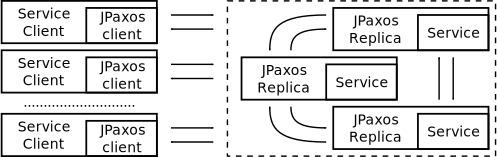
\includegraphics[width=0.44\textwidth]{architecture/userArchitecture1.pdf}
  &
  \hspace{0.02\textwidth}
  &
  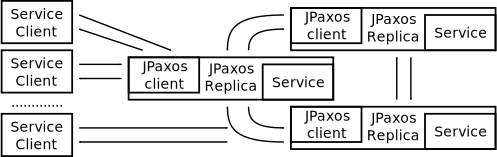
\includegraphics[width=0.44\textwidth]{architecture/userArchitecture2.pdf}
  \\ 
  \scriptsize a) JPaxos client integrated with service client
  & & 
  \scriptsize b) JPaxos client integrated with the replica\\
 \end{tabular}
 \fcmfcaption{Two models of JPaxos}\label{fig:jpaxos_processes}
\end{figure}

The JPaxos \texttt{Client} is responsible for connecting to replicas, providing availability of service as the replica connected with client crashes and ensures that the request will be eventually answered.

Integrating the \texttt{Client} module with service client provides full transparency of replication for the clients.
The service client contacts with the JPaxos \texttt{Client} module as if it would contact with the service -- i.e. it executes requests and gets answers for them.

If one chooses the second approach -- integrating \texttt{Client} in the replica -- the transparency is lost, and the programmer using JPaxos must care for selecting a working replica himself. However, this approach enables using JPaxos in wider context -- for example, one could possibly create a REST web service, and use an usual web client as the service Client, while the service itself would be replicated using JPaxos.

The JPaxos Replica module is responsible for global request ordering, passing the requests to the service, answering to the clients and recovering service from crash.

The service itself must be integrated within JPaxos replica. It gets the requests and responds to them. However, in order to make the resource usage bounded JPaxos requires additional functionality from the service, that partially breaks the transparency - the service must provide snapshots of it's state
once a time, % TODO: lepsze sformuowanie
as well as be able to recover it's state from a snapshot, possibly made by other replica.
As we assume that the services are deterministic, recovering from snapshot originating from other replica is not an issue, however for some services creating a snapshot may present a challenge.

\subsection{Client and client-replica communication}

The JPaxos client module is a single, small-weight module that performs several tasks:
\begin{itemize} 
 \item Connects to the replicated service
 \item Reconnects to the replicated service if the connection is lost (e.g. if a replica crashed)
 \item Retrieves (or acknowledges) a Client ID for recognising the requests
 \item Sends the requests
 \item Waits for answer, retransmitting the request if needed
\end{itemize}

For the communication with replicas Client uses TCP protocol.

\subsection{Service}

Service is the core part -- in fact it's the service that uses JPaxos for replication.
In order to connect a service with the library, it must implement an interface provided by JPaxos. The interface provides required communication between the library and the service.

The interface for interconnecting JPaxos replica and service allows for:
\begin{itemize}
 \item Executing requests and providing answers for them
 \item Creating Snapshots
 \item Recovering from snapshots
\end{itemize}

\subsection{Replica}

Replica is the most important part of the JPaxos. It consists of numerous modules as depicted on the figure \ref{fig:replica_architecture}.

\begin{figure}[h]
 \centering
 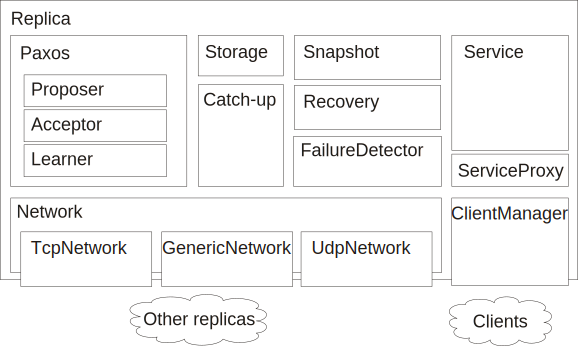
\includegraphics[keepaspectratio, width=0.75\textwidth]{architecture/replica_architecture.pdf}
 \caption{Block diagram of JPaxos modules}
 \label{fig:replica_architecture}
\end{figure}

Short description of the modules of JPaxos goes as follows:

\begin{description}
  \item[Replica ] interconnects other modules - especially the ClientManager, Paxos ans ServiceProxy
  \item[ClientManager ] maintains connection to clients, receives requests from them and forwards the answers
  \item[Paxos ] implements Paxos consensus algorithm
  \begin{description}
    \item[Proposer ] sends new proposes
    \item[Acceptor ] receives proposes and accepts them
    \item[Learner ] collects accepts and decides
  \end{description}
  \item[CatchUp ] takes care for lost ballots as well as retrieves the state from others on recovery
  \item[SnapshotMaintainer ] controls snapshot mechanism
  \item[Recovery ] chooses proper recovery method and does the actual recovery processes
  \item[Storage ] keeps the state of Paxos protocol - view number, log of consensus instances and snapshot
  \item[Service Proxy ] as only module contacts with the Service, provides as much transparency as possible for the service
\end{description}

\section{Storage and data structures}
\label{sec:storage_and_data_structures}

Apart of modules and interaction among them it is important to choose proper routines to access data. Both within modules as well as data shared across whole JPaxos.

\subsection{Process descriptor}

Every application has some configurable options that stay constant during the run. In JPaxos all these constants are kept in the \texttt{ProcessDescriptor} class.

During the startup JPaxos reads configuration file and initializes ProcessDescriptor with:
\begin{tightList}[\setlength{\labelwidth}{0em}]
 \item[\textbf{crashModel}] the crash model (see chapter \ref{chapter:recovery})
 \item[\textbf{logPath}] path for the stable storage
 \item[\textbf{localId}] the number of replica
 \item[\textbf{numReplicas}] count of the replicas
 \item[\textbf{windowSize}] preferred window size (see \ref{subsec:concurrent_instances})
 \item[\textbf{batchingLevel}] maximum size of the batch (see \ref{sec:batching})
 \item[\textbf{maxBatchDelay}] delay for connecting requests for batching
 \item[\textbf{network}] network protocol to be used
 \item[\textbf{maxUdpPacketSize}] threshold for generic network
\end{tightList}

\subsection{Storage interface}
\label{subsec:storage_interface}

\texttt{Storage} interface is responsible for holding the data for Paxos
protocol.

The data is shared across various modules.
It is very likely that various threads might want to access the Storage simultaneously. In order to prevent concurrency-related errors only one thread, dispatcher, may access these data. So if one wants to modify the \texttt{Storage}, a proper \texttt{Runnable} must be passed to the Dispatcher for execution (see subsection \ref{sec:threads}).

\paragraph{\normalfont \ttfamily lsr.paxos.Storage}
holds the data as follows:
\begin{tightList}[\setlength{\labelwidth}{0em}]
  \item[\textbf{log}] the Paxos Log (see the subsection \ref{subsec:the_paxos_log})
  \item[\textbf{view}] current view
  \item[\textbf{firstUncommitted}] first not decided yet instance.
  \item[\textbf{windowSize}] current size of the window used for multiple instances
  \item[\textbf{acceptors}] list of processes acting as acceptors
  \item[\textbf{snapshot}] most recent snapshot
  \item[\textbf{epoch}] current epoch vector (see section \ref{sec:epoch_ss})
\end{tightList}

\strut

The \texttt{Storage} implementation must be chosen according to the Recovery Model needs.
The implementation decides which elements must be kept on the Stable Storage and which may be placed in the volatile memory.

\subsection{The Paxos Log}
\label{subsec:the_paxos_log}
The most important for Paxos data structure, the Log, is part of the \texttt{Storage}.

In our program responsible for that is interface \texttt{lsr.paxos.Log} and class \texttt{lsr.paxos.Con\-sen\-susInstance}.

\texttt{ConsensusInstance} is class keeping all data related to single instance:
\begin{tightList}[\setlength{\itemindent}{0pt}\setlength{\leftmargin}{2\leftmargin}]
  \item[\textbf{state}] the instance can be in one of three state:
  \begin{tightList}[\setlength{\itemindent}{0pt} \setlength{\labelwidth}{7em}]
    \item[\texttt{\tiny UNKNOWN}] no information about the value of this instance
    \item[\texttt{\tiny KNOWN}] view and value are specified and \textbf{can} be changed later,
    \item[\texttt{\tiny DECIDED}] value is already chosen and \textbf{cannot} be changed.
  \end{tightList}
  \item[\textbf{view}] view of last received message related with this instance,
  \item[\textbf{value}] the value which is held by this instance (packed requests received from clients which are executed after deciding),
  \item[\textbf{accepts}] set of known replicas which accepted (view, value) pair.
\end{tightList}

Theoretically \texttt{Log} should contain all instances from the first up to the current one. Of course, the implementation cannot provide this. The log must however contain all instances between the oldest still needed and current one. Only method that guarantees bounding the log (i.e. that count of needed instances will stay finite) is the ability to record a state of the Service periodically -- we call this functionality snapshotting (see \ref{sec:snapshotting}).

\texttt{Log} implementation keeps always all instances with id between \textbf{lowestAvailableId}(inclusive) and \textbf{nextId} (exclusive). Instances below \textbf{lowestAvailableId} have already been truncated and instances above \textbf{nextId} are yet unknown.

New instances can be appended to log and after this operation \textbf{nextId} value is increased by 1. \\Log allows also to retrieve instances from it. There are 3 possible cases when retrieving instance with specified id:
\begin{itemize}
  \item (id $<$ lowestAvailableId) -- instance has been truncated and null value is returned,
  \item (lowestAvailableId $\leq$ id $<$ nextId) -- instance is inside log so it is returned,
  \item (nextId $\leq$ id) -- empty instances between nextId and id are created and empty instance is returned.
\end{itemize}
Old instances can be removed by truncating log and after that lowestAvailableId is increased. 

Appending, retrieving and truncating instances are three main operations performed by log.

Check if this is still correct:

\subsection{Significant data structures}
Other noteworthy data structures include:
\label{subsubsec:significant_structures}
  \begin{description}
    \item[pendingRequests Map\textless RequestId, ClientId\textgreater] Keeps the requests received from the client for execution that were not yet executed. After execution of request, the reply is sent to client from this structure.
    \item[lastReplies Map\textless ClientId, Reply\textgreater] For each client, keeps the last reply that was sent to it. If client retransmits message which was executed, replica responses immediately.
    \item[decidedWaitingExecution Map\textless Integer, BatchedRequests\textgreater] Paxos might decide instan\-ce $k$ before instance $k-1$, but the replica must execute all requests in order. So it must cache instance $k$ until all previous instances are decided.
    \item[executedRequests Map\textless ClientId, Reply\textgreater] We have to save IDs of all requests which were executed on state machine to prevent executing the same request twice.
	\item[executedDifference Map\textless Integer, ReplyList\textgreater] Used to recreate executedRequests structu\-re from moment when snapshot was made by state machine.
  \end{description}



\section{Threads}
\label{sec:threads}

Proper design of multi-threaded application must contain description of the major threads, their responsibilities and interactions.

\begin{description}
  \item[Replica] \hfill
    
    Designed as event loop -- the thread waits for new events at certain event queue and reacts on them.

    The event may either be signal from Paxos about new decision, or may concern snapshotting -- new snapshot was made by service, catch-up provided new snapshot or new snapshot is requested from the service.

    For most of the time Replica thread waits for requests to be ordered. If they can not be yet executed, puts them on a list (uses for that the decidedWaitingExecution object).
    
    As for snapshotting -- replica is a proxy ensuring linearizability in snapshot handling.
    Multiple threads (replica itself, dispatcher and catch-up) may therefore safely execute their snapshot-concerning routines.
    
  \item[Dispatcher] \hfill
    
    Also designed as an event loop, the dispatcher executes Paxos consensus algorithm as well as provides secure access to critical data structures -- to the \texttt{Storage} (see subsection \ref{subsec:storage_interface}).
    
    The Dispatcher thread actually is using a priority queue, so that the events are sorted by their importance -- for example, writes to the storage and Paxos-related processing has higher priority than the Catch-Up tasks.
    
    It is responsible for sending, receiving and handling most of the protocol messages as well as accessing the \texttt{Storage} and triggering Catch-Up.
    
    Events are placed on the event queue in the following situations:
    
    \begin{tabular}{rl}
      Recovery.NetworkListener & \begin{tabular}[t]{l}
                          received a new message \\
                          sent a message
                        \end{tabular} \\
      FailureDetector & \begin{tabular}[t]{l}
                          suspects another process \\
                          leader sends alive messages
                        \end{tabular} \\
      Paxos.NetworkListener & \begin{tabular}[t]{l}
                          received a new message \\
                          sent a message
                        \end{tabular} \\
      Paxos.propose() & \begin{tabular}[t]{l}
                          the application starts a new proposal
                        \end{tabular} \\
      Paxos.startProposal() & \begin{tabular}[t]{l}
                                the application asks the current process \\ \hspace{1em} to become a proposer.
                              \end{tabular} \\
      Proposer &  \begin{tabular}[t]{l}
                    timeout for requests to be batched
                  \end{tabular} \\
      Retransmitter & \begin{tabular}[t]{l}
                        message should be retransmitted
                      \end{tabular} \\
      Catch-Up &  \begin{tabular}[t]{l}
                   gets and merges log fragment \\
                   a message is received \\
                   received a snapshot form other replica \\
                   a periodcal catch-up should occur
                 \end{tabular} \\
      SnapshotMaintainer & \begin{tabular}[t]{l}
                             truncates the log after receiving new snapshot
                           \end{tabular} \\
    \end{tabular}


	\item[NioClientManager] \hfill

		Using java.nio package we need only one thread \textsc{SelectorThread} to manage all clients connection. Every time new event occurs (incoming connection waits for accepting, data received from client, data ready to be sent) appropriate action is executed. Current implementation allows easy scaling to more \textsc{SelectorThread}'s to balance the CPU load if one thread wouldn't cope with big number of connections.

	\item[UdpNetwork] \hfill

		One thread responsible for listening on DatagramSocket for datagram packages. Every time new message is received, it is deserialised and all listeners are notified. 

	\item[TcpNetwork] \hfill

		For TCP connection between each two replicas a separate thread for receiving and transmitting is created. Also there is one thread which waits for new incoming connections. Overall we have  $2 \cdot replica\_count - 1$ threads handling TCP. Each of them can be in one of three states:
		\begin{itemize}
			\item connected, waiting for new messages,
			\item not connected, trying to establish new connection,
			\item not connected, waiting for new connection to be established by other replica.
		\end{itemize}
\end{description}

\chapter{Implemented Features}

In this chapter we present the implementation details of some non-trivial modules.

\section{Granting unique request IDs}

A request must be distinguishable from any other request. Only this guarantees that we will be able to say if a request is retransmitted, or it's a new one. A common method is to split the request identification in two parts: the client ID and sequential number. As far as assigning sequential number is trivial, method providing unique client IDs must be carefully chosen, especially taking under consideration the crash-recovery model.

The client ID has to be unique for two different clients. To guarantee this, replicas must be responsible for granting IDs to clients, because a client has no knowledge of other clients ID.

Below we present some of the possible methods for solving this problem:

\paragraphNewline{Based on number of replicas}
Each replica can grant numbers incremented by number of replicas, starting from ID of local replica. For example, if we have three replicas, replica with ID 0 can grant numbers 0, 3, 6, 9, \ldots{} and replica with ID 2 can grant 2, 5, 8, \ldots{} . It guarantees that two different replicas will not grant the same ID. This solution works with crash-stop and crash-recovery with stable storage. This will not work when replica can recover from crash without stable storage, because it doesn't know what was the last granted ID.

\paragraphNewline{Time based}
This is different approach -- we use system time as the source of unique numbers. To each client ID we are adding also information when replica was started (in milliseconds).

For example, if a replica has been started at time $t$, it will grant for new clients IDs $(t + $\textit{localId}$)$, $(t + $\textit{localId}$ + n)$, $(t + $\textit{localId}$ + 2n)$ \ldots

This method assumes that local system timer is not set back into past and also that replica will not recover in the same millisecond. If these assumptions are fulfilled, then unique IDs are guaranteed also in crash-recovery model without stable storage. This approach is currently default in our library.

\paragraphNewline{View based}
Because time based assumptions sometimes cannot be guaranteed, another approach for crash-recovery model may be considered. Instead of adding information about start time, we can add current view number. In each view, there is exactly one leader -- so after the prepare phase this replica can grant clients IDs as pair (view, sequence number). Two different replicas cannot start the same view.
Also we have to guarantee that only leader replica after prepare phase can grant new client IDs.

This approach will also work by using the Epoch numbers -- if a leader crashes, the view must be increased by his recovery.


\section{Catch-up}
\label{sec:catch_up}

\paragraphNewline{Motivation}

Paxos must guarantee that every valid replica will eventually decide. Most papers about Paxos state that if a replica notices lack of activity for some instance, it must send new proposal and eventually decide. But by using view for all instances, this would mean often view changes -- and this contradicts performance.

Therefore a different approach is used by us. Notice, that if the leader is correct, it will decide. If it crashed a new leader will be elected. If the leader is correct, and no activity about an instance is noticed, that means the value is already decided and the replica is in the minority that does not know about the decision.

In such case, instead of forcing a new proposal, we use the Catch-up module.
The Catch-up has to download all missing decisions. This solution is faster than restarting the ballot if it is already decided and it also does not need a view change.

\paragraphNewline{Recovery}

This module is also used by recovering the replica -- as a tool for downloading all decided instances up to required state.

But there is one drawback -- for the recovery one needs to know also instances yet undecided.  However, if the system is operational, after a short time all required instances will be decided. If the system is not operational the recovery cannot converge. So downloading only decided instances is correct, but may cause small delay by recovering

\subsection{Log-based vs state-based recovery}
\label{subsec:log_based_state_based_recovery}
A replica can catch-up either by copying the missing decisions or by a combination of transferring the state plus the most recent decisions.

In the rest of this paper \emph{log-based recovery} refers to the first option while \emph{state-based recovery} refers to the second option.

One should use of course the method achieving better performance. But which method is faster depends on the particular characteristics of the system:

\begin{description}
  \item[Size of the state] For services with large states  it is better to avoid transferring the state as much as possible. On the other hand, if the service state is small, transferring it might be better. In the extreme case, the service state is of a similar size or smaller than a single command. In this case, it would always be better to transfer the state.

  \item[Execution overhead] Executing commands takes some processing time which is not required when transferring the state. Therefore, even if the service state is bigger than the corresponding commands, it might be faster to transfer the state.

  \item[Bandwidth available] With limited bandwidth, the fastest  method will likely be the one that transfers less data. Otherwise, the execution overhead will likely be the dominant factor.
\end{description}

\paragraphNewline{State-based recovery time}

State-base recovery has the following steps:

\vspace{-0.5em}
\begin{center}
  \footnotesize
  \begin{tabular}{ll}
    Serialisation               & state is transformed into a sequence of bytes \\
    Transfer                    & size is sent via network \\
    Deserialization             & state is rebuilt at destination \vspace{0.5em} \\
    Residual log-based-recovery & recovery from snapshot process is made \\
  \end{tabular}
\end{center}
\vspace{-0.5em}

The first three tasks may be done concurrently. Assuming that the fourth task is comparatively fast, we can consider that the total recovery time is the maximum time it takes to do each of the first three tasks.

\paragraphNewline{Log-based recovery time}

Log-based recovery consists only on sending the commands and executing them at the replica. Once again, sending and executing can be done concurrently, so the total duration is the max of the time it takes to transfer all the updates or to execute them.

\subsection{Conditions for starting and finishing the catch-up}
\label{subsec:conditions_for_starting_and_finishing_the_catch_up}
Many possible rationales may be used as indicator when the process should begin the catch-up. Also conditions needed for the stop process are a significant issue.

\paragraph*{Starting catch-up}
Activating the mechanism should not happen too early, that is when Paxos itself is still able to take the decision -- target of catch-up is to complement decisions missing due to packet loss. On the other hand late initiating leads to delaying command execution, and thus significant performance loss.

Most common events used to initialise the algorithm are:
\begin{itemize}
  \item No traffic for the ballot during a particular period of time (\textsc{timeout})
  \item An instance with higher ID (i.e. newer instance) has already been decided \\ (\textsc{higher instance decided})
  \item Instance with ID higher than $\alpha$ has been started, and the implementation ensures that only instances up to $\alpha$ are started as $\alpha-ws$ stays undecided (\textsc{window})
  \item Activate periodically the mechanism (\textsc{periodical})
\end{itemize}

These methods let the replica suspect, that a locally undecided instance has already been decided, so its log state is not up to date. It's good to use more than one of them, as each method is sensitive for a particular scenario, perhaps performing bad otherwise.

Simplest, but not efficient for most uses is the \textsc{periodical} method -- it guarantees that from time to time the replica will be up to date.
Too often used may cause bandwidth and processor consumption, too rarely -- having old state for unacceptably long time.

The \textsc{timeout} event is caused either if problems with network occur, or if the \accept messages were lost -- otherwise current leader and other replicas would generate traffic for the ballot. The replica should try to learn the state of voting in such case, otherwise as long as no new proposal will arise, the replica will have old state.

\textsc{higher instance decided} means that a later started voting already finished. We may assume the previous voting took similar amount of time -- that is, it should be already finished. Message loss or varying latency can also cause the situation that a newer consensus is decided as the older is still in progress. To avoid this situation the method may be extended to: if the number of newer decided instances exceeds a constant value, then the catch-up should be initiated.

The method, as well as the earlier described, may be used in case when operations on state machine require long processing. Risk of loosing small bandwidth for catch-up may be small enough compared to earlier arrival time of resource-consuming task.

The \textsc{window} method is only one guaranteed, because of it's assumption: the algorithm uses window of maximum size $ws$. If the condition that all decisions outside the window must be decided is violated on one replica, it means that other replicas, at least current leader, already decided the instance. This means no new messages concerning the ballot will emerge, and catch-up is necessary.

A different problem is when a replica doesn't know that the instance already exists (for example, a short-time netsplit or bad luck caused all messages for the replica to be dropped). In this case, the catch-up should be started as well. 
Either periodic requests must be sent, or additional information must be acquired. It should be emphasised, that as any newer ballot starts, the replica is informed about the existence of missing instance. 

Although this is not critical, it prevents state machine from executing the command until new instance emerges. That means performance loss, as the old command must be caught-up and executed before the new.

In our system, replica is notified about highest instance id from \alive message from leader. The leader is attaching this number to every \alive message sent. This guarantees that every replica learns what instances already exists within failure detector timeout.

\paragraph*{Stopping catch-up} As the algorithm runs, the state of Paxos may not be stable, i.e. new ballots may start. Therefore selecting the moment when catch-up should be deactivated is not trivial.

One method is to calculate conditions a priori (for example the IDs of missing instances), and continue the process as long as needed. But this can easily lead to a constant switching on and off the catch-up -- voting for new instances may be faster than catching up, so as the predefined conditions are met, new event already caused catch-up activation.

The better solution is to determine dynamically if catch-up is still needed. Method that seems most convenient for that is checking, if all instances outside the window are already decided. Stopping earlier is bad, as we know that at least the current leader must have decided for the missing instances, and that means we will not get the value via Paxos algorithm.

Finishing the catch-up process later, that is requiring any messages in the window to be decided is also not a good solution -- unless we have some additional knowledge that the instance has already been decided (for example, leader's last uncommitted instance ID is sent in \propose or \alive messages).

Problem arises, if there really were decided instances inside the window. If there are no new ballots, arrival time of these requests will be delayed. In our opinion, the problem is not that severe, especially if window size does not exceed reasonable size.

\subsection{Transport protocol}
\label{subsec:transport_protocole}
As totally separate from Paxos, the catch-up may use different transport protocol than the consensus algorithm.
Choice of transport layer must take into account characteristics of this mechanism as well.

Both TCP and UDP may be used -- both having their pros and cons, presented in table below

\begin{center}
\small
\begin{tabular}{>{\raggedleft\hspace{0pt}}m{0.47\textwidth}m{0.47\textwidth}}

\multicolumn{1}{c}{ \textbf{TCP} }& \multicolumn{1}{c}{ \textbf{UDP} } \\ 
automatic retransmission guaranteed by protocol &
                                retransmission must be implemented manually \\ 
flow control provided by protocol & no flow control, it \emph{is} easy to congest network \\
big messages automatically fragmented, mer\-ged and managed &
                                splitting and handling big messages must be~self implemented \vspace{0.5em} \\

request cannot be changed at retransmission &
                                request can be changed each retransmission \\
default retransmission time & custom retransmission time \\
another message may be sent once the previous was delivered &
                                new datagram may be sent anytime, no matter if the previous reached the target \\

\end{tabular}
\end{center}

When catch-up is needed,  our network must have (probably high) message loss. That means catch-up messages may also get easily lost.

We have noticed, that it is more efficient to use UDP for all smaller messages -- if the package gets lost, we're retransmitting it with updated query. Sometimes even twice retransmitted UDP message is faster than one TCP. In TCP, the timeout for ACK message grows automatically - and that may cause big delays. During experiments, with 30\% message loss, transmitting a message using TCP smaller than UDP-datagram size took even more than 4 seconds to reach the other side.

In UDP, single message delay or loss does not block communication to the replica -- but in TCP does.
In this case no new catch-up query may be sent to this replica, as long as the previous will be processed. The request cannot of course be changed. It means that once we got the response, core protocol may have already missed another instances to catch-up.

\subsection{Requirements}
\label{subsec:catch_up_requirements}
The speed and resource consumption must be correctly balanced.

In theory, catching-up can be delayed any finite time. On the other hand, it is important for view changes and for bounding the size of the log. A view change will take longer if the new leader is missing many requests. Since during a view change no new requests are being satisfied, we need to keep its length as short as possible. Additionally, if a replica doesn't know instance $i$, it cannot execute any request higher than $i-1$. This also means that it cannot remove entries from the log.

In practical approach most significant requirements for catch-up are: good performance and small resource usage. For sure catching up should not slow down the core protocol.
Good performance demand has one main reason: arrival time of the tasks for state machine is dependent on being up to date. If catch-up would get information too late, the state machine would get long list of, possibly high CPU-consuming, tasks at once, instead of doing them in spare time before.

Therefore, it is desirable to catch-up as often as possible, but without slowing down the service significantly.

It should be noticed, that only the followers will have to catch-up, since the primary learns of all previous decisions on a view change and then is the one proposing new values and leading the protocol.

\subsection{Catch-up algorithm}
\label{subsec:catch_up_algorithm}
The catch-up algorithm should contact other replicas and copy the decisions that are not known. Question when this should be done is discussed in section \ref{subsec:conditions_for_starting_and_finishing_the_catch_up}. Here the main idea of JPaxos catch-up algorithm is presented.

To activate the catch-up, we use \textsc{window} and \textsc{periodical} methods (see \ref{subsec:conditions_for_starting_and_finishing_the_catch_up}). The leader also sends by each \alive message the information about highest started instance.

This ensures that the replica will catch-up eventually, even if there are no new requests, and that a replica never stays too much behind the others, at most \textit{ws}.

There are three messages that may be sent during the algorithm: \catchUpQuery[], \catchUpResponse and \catchUpSnapshot[].
\begin{description}
 \item[\normalfont\catchUpQuery] Request for missing instances. Carries list of missing ID's and may have one of the two flags set: first flag indicates if this was a periodical catch-up, second -- if we want to get last snapshot, not missing log fragment.
 \item[\normalfont\catchUpResponse] Response sent for every received request. Has list of decided instances for requested numbers. The list may be empty. This message may have two flags: either if the query had periodical flag set, or indicator that the replica doesn't have old enough log, and state transfer is the only possibility.
 \item[\normalfont\catchUpSnapshot] If another replica asked for our last snapshot, this message is sent. It contains only responders last snapshot.
\end{description}

The list describing missing instances is constructed quite simple: it contains all undecided instance numbers plus the (highestID+1) as the first instance replica has no knowledge about. The responder sends therefore all decided from the list + all decided instances higher or equal than the additional number.

In order to make the messages smaller, a trick has been used: the list contains of two lists. One called range list and the other instance list.
Range list contains intervals we miss, while instance list -- single numbers. For example, if we would miss instances 1,2,4,6,7,8,9,11, and the highest instance we know is 12 (state decided) our lists would look like:
\begin{quote}
$[\langle1,2\rangle; \langle6,9\rangle]; [4,11,13]$
\end{quote} 
Notice the number 13 -- it's the first we have no idea of existing, as mentioned above.

Catch-up works as follows:

\begin{algorithmic}[1]
  \REPEAT
    \STATE \label{alg_1_a} Choosing target replica
    \STATE Creating list of missing instances
    \STATE Send a \catchUpQuery
    \STATE \label{alg_1_b} Wait for timeout or for response
  \UNTIL{\label{alg_1_c} catch-up succeeds}
  
  \vspace{0.5em}
  
  \STATE \textbf{upon} receiving \catchUpQuery \textit{query}
    \IF{\textit{query} has snapshot flag set}
      \STATE Get last snapshot
      \STATE Prepare \catchUpSnapshot message
      \STATE Send the message
    \ELSIF{requested instances already not in log}
      \STATE Send \catchUpResponse with \textit{snapshot} flag
    \ELSE
      \STATE Gather all decided instances
      \STATE Send \catchUpResponse
    \ENDIF

  \vspace{0.5em}
  \STATE \textbf{upon} receiving \catchUpResponse \textit{response}
    \IF{\textit{response} has \textit{snapshot} flag set}
      \STATE Prepare \catchUpQuery with snapshot flag
      \STATE Send the query
    \ELSE
      \STATE Merge received log (if any)
      \STATE Wake up the Catch-up loop (line \ref{alg_1_b})
    \ENDIF
  
  \vspace{0.5em}
  \STATE \textbf{upon} receiving \catchUpSnapshot \textit{snapshot}
  \STATE Check if \textit{snapshot} is newer than current one
  \STATE Replace the current snapshot with \textit{snapshot}
  \STATE Truncate logs (to stop catch-up)
  \STATE Wake up the Catch-up loop (line \ref{alg_1_b})

\end{algorithmic}

\vspace{1em}

In line \ref{alg_1_a} a best replica is chosen. We've implemented it as follows: a rating for each replica is kept. When sending a message, the rating decreases; when receiving response -- rises. If an empty response is received (except for \textsc{periodic} mode), we request asking the leader next time. Best replica for us is a follower with highest positive rating, or the leader if all followers have negative rating.

Magic line \ref{alg_1_c} executes a predicate checking if the catch-up shall finish (see \ref{subsec:conditions_for_starting_and_finishing_the_catch_up}).

\section{Snapshotting}
\label{sec:snapshotting}
As presented before, the support of storing and transmitting state of replicated machine is very useful and important part of a replica. In practical systems it is necessary -- it allows log truncating, faster recovery and catch-up.

\subsection{When to snapshot}
\label{subsec:when_to_snapshot}
Snapshots are needed in two cases: to enable catch-up and recovery, and to truncate the log. For both uses there is a different \textit{best moment} for making snapshot.

As for recovery, we get best recovery result if the snapshot would be done every executed order.
This, of course, is not the solution. It would completely decrease the throughput -- snapshot creation is resource-consuming.

For the catch-up the moment when another replica requests snapshot is the best for creating one. However, we should not demand creating snapshot when we want to, so it's better to rely on the service programmer.

For truncating the log snapshot should just be created periodically, without any additional requirements.

Therefore we assume the snapshot should be made when the cost of catch-up from log becomes bigger than cost of catch-up from snapshot.

Please notice, that catch-up time also includes time of state/log transfer.

\subsection{Replica vs state machine responsibility}
\label{subsec:replica_vs_state_machine_responsibility}
There are two approaches to the problem who is in charge with snapshot creation. Either the replica issues a snapshot, or the state machine chooses appropriate moment and forwards the state to replica.

Embedding this functionality into the replica will surely provide more secure work (state machine may simply not deliver the snapshots, what means forever growing log). It is easier for replica to measure size of the messages that should be transferred in order to catch-up (or recover).

However, the replica does not now anything about state machine. We can also assume, that the service is not aware of network conditions. Therefore choosing the proper moment (when cost of log-based catch-up becomes more expensive than state-based catch-up) is impossible for both. It is clearly visible, that state machine is better informed - it knows not only the size of requests, but also may estimate size of it's current state and resources needed to execute all commands from log.

The latter is most significant difference: replica has no idea how long the log execution from previous snapshot would take. It seems possible to estimate this: measuring time between request and replay might solve the problem. But such estimate can give mistaken result, especially in multi-process environment. If another process is consuming CPU, or the replica waits a long time for granting some resources (like access to a file or even a printer), the estimate surely will not reflect real value.

Table below presents in compact way state of knowledge needed to select best moment for next snapshot:
\begin{center}
% use packages: array
\small
\begin{tabular}{r|c|c|}
\cline{2-3}
 & State machine & Replica \\ \hline 
\multicolumn{1}{|r|}{Size of requests} & known & known \\ \hline
\multicolumn{1}{|r|}{Size of state } & known & estimate \\ \hline
\multicolumn{1}{|r|}{Log execution time} & good estimate & poor estimate \\ \hline
\multicolumn{1}{|r|}{Time for sending message} & unknown & estimate \\ \hline
%\multicolumn{1}{|r|}{ × } & × & × \\ \hline
\end{tabular}
\end{center}

\subsection{Our approach to snapshotting}
\label{subsec:our_approach_to_snapshotting}
Snapshotting, as described above, may be done in a variety of ways. Also how often the snapshots are made depends on implementation. Here we give main clues how the snapshotting is implemented.

The decision who orders a snapshot creation has been left to the future user of the library. To achieve this, some assumptions has been taken -- mainly
concerning architecture of the service.

The service must implement three methods: \texttt{askForSnapshot}, \texttt{forceSnapshot} and \texttt{up\-date\-To\-Snap\-shot}. Also it is required to implement adding and removing snapshot listeners -- objects that implement \texttt{onSnapshotMade} function. When a snapshot is made on the state machine, method \texttt{onSnapshotMade} with the snapshot as parameter must be called on all snapshot listeners.

Replica measures size of the log after every n-th instance, and calculates average size of the snapshot basing on previous ones. By every log measurement a ratio is calculated: $\frac{ \text{log size} }{ \text{snapshot estimate} }$. As the ratio exceeds one constant, method \texttt{askForSnapshot} is called. After another constant \texttt{forceSnapshot} is executed.

There are several approaches possible on who decides proper time for the snapshot:
\begin{description} 
 \item[State machine only] -- service ignores the functions \texttt{askForSnapshot} and \texttt{forceSnap\-shot} and does the snapshot on its will.
 \item[Using replica calls as hints] -- service takes under consideration \texttt{askForSnapshot} and \texttt{fo\-rce\-Snapshot} functions, but decides itself when to do snapshot
 \item[Balanced responsibility] -- service uses both \texttt{askForSnapshot} and \texttt{forceSnapshot}; the first as a hint, the latter treats as an order
 \item[Replica only] -- each time \texttt{askForSnapshot} is called, the state machine does snapshot
\end{description}

Snapshotting requires also additional data exchanged between replica and service: the state machine must know the request number, in order to let snapshot identification in replica. For example, if the snapshotting would be done completely on service's side, how would the replica know after which command the snapshot was taken.


\section{Batching}
\label{sec:batching}
Batching means using the same consensus instance to order several requests.

This optimisation does not need any changes to the Paxos algorithm, only requires that requests from one instance can be ordered deterministically by replica, so that replicas know the order in which they should execute the requests. That is no problem, as a byte stream is already ordered -- so each replica will decode the requests the same way.

To achieve multiple requests in the same instance an additional activity must be taken up by proposer and later, by replica, just before execution.

The proposer needs to \textit{stick} together the requests, and from that moment on they are treated as one. The other part, dividing it again into requests, should be done after the decision has been taken.
\begin{figure}[h]
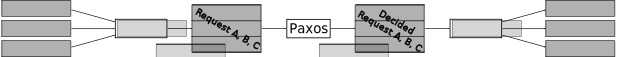
\includegraphics[keepaspectratio, width=\textwidth]{features/batching.pdf}
\vspace{-1em}
\caption{The batching mechanism}
\vspace{-1em}
\end{figure}

As the count of concurrent instances is bounded (see subsection \ref{subsec:concurrent_instances}), without batching every client needs to wait for his own instance. With batching many client requests may be \textit{packed} in one instance. That, on one side, increases the throughput and decreases the delay.
On the other side, message size is getting bigger -- and that means slower voting.

Here arises a question: how many requests to batch? One boundary is quite obvious -- serialized message should not be bigger than transport protocol frame size. As for UDP the size is about 65kB, but for TCP stays unbounded.

From the benchmarks %TODO: referenc on nuno (?)
we can see that best performance and latency is achieved as the batching size is set to the minimal size when all available bandwidth is used.

Another problem concerns the proposer: should there be a lower limit of requests in one instance? Doing so we require waiting for new clients to come. Not waiting means sometimes severe throughput loss.

If we had a single request only, just waiting for an other would cause endless waiting. So a timeout is needed here.

If we decide not to wait at all -- we're packing all the proposer got until now into a single request (if it fits, of course). Such approach guarantees good behaviour if the system state is not changing -- under load, usually we're unable to pack all requests we got, while with small amount of requests no delay by packing decreases the latency.

Both batching size and the timeout for gathering requests in batch is configurable in our library.

\section{Service Proxy}
\label{sec:serviceProxy}

Some operation on service require proper arguments. Should a service be responsible for that? Batching causes that the snapshot can be made after full instances, and not after each request. Should a service take care  for that?

This is not desired. We want to provide as much transparency as possible, without forcing the service to remember redundant data.

\texttt{ServiceProxy} is a module that translates JPaxos instances to Service requests and takes care for all the requirements concerning snapshotting. From Replica side, interaction with the Service through \texttt{ServiceProxy} is instance-oriented and convenient. From Service side, the interaction with clients is as transparent as possible.

To achieve this the \texttt{ServiceProxy} keeps list of responses for all requests since the previous snapshot as well as information required later to restore proper request sequential number from a snapshot.
As the replica provides a snapshot, this module adds to the snapshot required data.

Overhead caused by this proxy should be smaller than the difference in speed of the service if the service were to be aware of instances. The difference is size of the snapshot depends on the state size, but usually the state is much bigger than a few responses required to provide transparency.

Of course, this does not release the service from responsibility of providing valid snapshots. The service still must provide corresponding request sequential number for the snapshot it creates.

\chapter{Recovery}

\section{Crash stop}
\label{sec:crash_stop}

\section{Crash-recovery with stable storage}
\label{sec:full_ss}

\section{View based recovery}
\label{sec:view_ss}

\section{Epoch based recovery}
\label{sec:epoch_ss}

\chapter{Conclusions}

%Zakończenie pracy zwane również Uwagami końcowymi lub Podsumowaniem powinno zawierać ustosunkowanie
%się autora do zadań wskazanych we wstępie do pracy, a w szczególności do celu i zakresu pracy oraz
%porównanie ich z faktycznymi wynikami pracy. Podejście takie umożliwia jasne określenie stopnia
%realizacji założonych celów oraz zwrócenie uwagi na wyniki osiągnięte przez autora w ramach jego
%samodzielnej pracy.
%
%Integralną częścią pracy są również dodatki, aneksy i załączniki np.~płyty CDROM
%zawierające stworzone w ramach pracy programy, aplikacje i projekty.

In this thesis, we have studied the problem of state machine replication based
on Paxos algorithm defined in \cite{Lam98}. We described challenges faced in
implementation phase to make the library ready to use in production systems
with support of crash-recovery model, message loss and communication delays.

We first presented the Paxos algorithm with theoretical background. Then we
focused on problems which occurs when transforming one page pseudocode of
distributed algorithm to few thousands line of production code. We presented
the architecture of our library with short description of every module and data
structures used. The library have to handle unreliable network with message
loss and delays, so we presented the catch-up mechanism which guarantees that
eventually every correct replica will be up to date. By introducing snapshot
mechanism, we solve a problem with infinite grow of log. To make the library
very efficient, we implemented several performance improvements like concurrent
instances, skipping redundant message and batching. To tolerate crash-recovery
model, four different recovery algorithms has been implemented and described in
this paper.

To test the library we implemented replicated hash map as an example of
deterministic service. We used it to verify that our library is working
correctly and that API we provide is user friendly. Our library is used as 
communication layer in PaxosSTM master thesis \cite{Tad10}.

Our future work includes further performance improvements to Paxos protocol and
implementing more crash-recovery algorithms with no use of stable storage.  It
would be also interesting to evaluate all recovery algorithm in network with
message loss and environment when failure of replica is a common scenario.
Finally we would like to publish the library as open source project and test it
in production environment.

%In this thesis, we have studied the problem of computing the "worthiness" of
%data items for each peer in unstructured P2P networks where the "worthiness" of
%an item is defined as in [SNW08]. We presented techniques for a better
%estimation of these values.  As a result, a more eficient solution for the P2P
%replication problem defined in [SNW08] is achieved.  
%
%We first studied the problem in a centralized environment, where all parameters
%of the network are known to each individual peer, and provided a method based
%on Chapman- Kolmogorov equations to eficiently compute the worthiness of data
%items in a such environment. As the main result of this thesis, we have
%presented a fast distributed algorithm to eficiently compute the "worthiness"
%of data items in the network. Our experimental evaluations on random graphs
%show that our algorithm converges much faster than the counting algorithm, but
%requires messages with larger (but still accept- able) size. In our algorithm,
%the informations regarding the query path starting from the query originator
%and the location of requested data items on this path are maintained and
%piggybacked the original query. Our algorithm incures O(kmn 0) space cost at
%each peer i where k is the maximum length of random walks, m is the number of
%data items stored in the network and n 0 is the number of peers in the
%k-neighborhood of i. There- fore, there is a trade-of between the time need for
%achieving a good estimation of the worthiness of items and the size of messages
%to be issued in the network.  
%
%Our future work includes computing worthiness of data items in a more eficient
%way i.e. in terms of number of messages, the size of messages to be issued in
%the network and the storage space which is needed at each peer to maintain the
%transition probabilities.  It would be also interesting to evaluate the
%eficiency of the algorithm on networks with heterogeneous parameters (e.g.
%query rates, network topologies) and with data of real P2P networks. Finally,
%further extensions and generalizations of the algorithm and considering other
%constraints of real P2P networks would be some directions of our future work.



% All appendices and extra material, if you have any.
\cleardoublepage\appendix%
\newcounter{pageTemp}
\setcounter{pageTemp}{\value{page}}
\pagenumbering{roman}
\chapter{JPaxos user guide}

\section{Overview}
\label{overview:overview}\label{overview::doc}\label{overview:jpaxos-user-guide}
JPaxos is a Java library and runtime system for efficient state machine
replication. With JPaxos it is very easy to make a user-provided
service tolerant to machine crashes. Our system supports the \emph{crash-recovery}
model of failure and tolerates message loss and communication delays.
\begin{description}
\index{State machine replication}\item[{\href{http://en.wikipedia.org/wiki/State\_machine\_replication}{State machine replication}}] \leavevmode\phantomsection\label{overview:term-state-machine-replication}
is a general method for implementing a fault-tolerant service by
replicating it on separate machines and coordinating client interactions
with these replicas (or copies). The physical isolation of machines in
a distributed system ensures that failures of server replicas are
independent, as required. As long as there are enough of non-faulty
replicas, the service is guaranteed to be provided.

\end{description}

JPaxos makes the following assumptions about the replicated service:
\begin{itemize}
\item {} 
deterministic behaviour, i.e. multiple copies of the service begun in
the start state, receiving the same inputs in the same order will
arrive at the same state having generated the same outputs

\item {} 
non-Byzantine failures, i.e. a service machine can only crash

\item {} 
crash-recovery supported, i.e. after crash, the service can be restarted
with the same IP address.

\end{itemize}


\subsection{Two execution modes}
\label{overview:two-execution-modes}
JPaxos can be run in one of the following two modes of operation
(the mode is set up from the configuration file at system start up
and cannot be changed at runtime):

Basic mode
\begin{itemize}
\item {} 
to be able to tolerate $f$ faulty replicas, the system must consists
of at least $2f + 1$ replicas (i.e. $n \ge 2f + 1$)

\item {} 
after replica crash, it recovers its state from other replicas

\end{itemize}

Extended mode
\begin{itemize}
\item {} 
no limit on the number of faulty processes (i.e. $f = n$)

\item {} 
after replica crash, it recovers its state from non-volatile memory

\item {} 
around 200 times slower than the basic mode

\end{itemize}


\subsection{Simple API}
\label{overview:simple-api}
For the end user JPaxos provides:
\begin{enumerate}
\item {} 
\code{Service} interface -- it specifies a few methods for interfacing
the user-defined service code with JPaxos; our library provides
abstract classes implementing \code{Service} interface, making it easier to
to create a new service (state machine);
see {\hyperref[api:jpaxos-service]{\emph{Service interface}}} for details

\item {} 
\code{Replica} class -- that should be instantiated and started
(see {\hyperref[api:jpaxos-replica]{\emph{Replica}}} for details)

\item {} 
\code{Client} class -- the part that may send request to be executed
(see {\hyperref[api:jpaxos-client]{\emph{Client}}} for details)

\end{enumerate}

The \code{Service} and \code{Replica} are bound to each other, while
\code{Client} can be located anywhere.

JPaxos guarantees that in crash-recovery model, with static groups,
lossy network with any delays:
\begin{itemize}
\item {} 
if the client sends a request, it'll eventually get the answer

\item {} 
every replica will execute the request exactly once

\item {} 
any two replicas will execute the requests in the same order

\end{itemize}


\subsection{Distributed implementation}
\label{overview:distributed-implementation}
JPaxos is a fully distributed implementation, which means that there
is no predefined central coordinator that might be a bottle-neck or a single
point of failure in the system.

For this, JPaxos implements
the \href{http://en.wikipedia.org/wiki/Paxos\_algorithm}{Paxos}
distributed algorithm with various optimizations, in order to efficiently
deliver client requests to all service replicas despite any failures.
Replicas receive all requests globally ordered, thanks to
the total-order (or atomic) broadcast protocol implemented on top
of Paxos.

Figure below shows processing of a single request message submitted
by the Client to the replicated state machine:
\begin{quote}
\begin{figure}[htbp]
\centering

\scalebox{0.500000}{\includegraphics{user_guide/state_machine.pdf}}
\end{figure}
\end{quote}

where \emph{Client} is an instance of the \code{Client} class, while \emph{s1}, \emph{s2},
and \emph{s3} are instances of the \code{Replica} class.

If a request is delayed or lost due to the network or replica failure,
after a timeout, it will be reissued by the \emph{Client}, as illustrated in
Figure below:
\begin{quote}
\begin{figure}[htbp]
\centering

\scalebox{0.500000}{\includegraphics{user_guide/state_machine_crash.pdf}}
\end{figure}
\end{quote}


\section{Deployment and configuration}
\label{config:deployment-and-configuration}\label{config::doc}
This section presents quick overview on what is necessary to compile the
library and how to configure the system and start the example which is included
in the distribution.


\subsection{Deployment requirements}
\label{config:deployment-requirements}
JPaxos requires the following components to be installed on the target system:
\begin{itemize}
\item {} 
\href{http://www.java.com/}{Java JRE 1.5} or later

\end{itemize}

Additionally, the following are optional but helpful tools in compilation and
packaging:
\begin{itemize}
\item {} 
\href{http://ant.apache.org/}{Apache Ant} -- used to run all build scripts (distributed under the Apache
License 2.0)

\end{itemize}


\subsection{Configuration file}
\label{config:configuration-file}
The format of configuration file used by \code{Configuration} class is the same as
default Java Properties file. As mentioned earlier, this file contains
nodes configuration and replica related options.


\paragraphNewline{Node configuration}
\label{config:node-configuration}
A node is configured with a single line containing \code{hostname}, \code{replica
port} and \code{client port}, separated with commas:

\begin{Verbatim}[commandchars=@\[\]]
process.@textless[]id@textgreater[] = @textless[]hostname@textgreater[]:@textless[]replica@_port@textgreater[]:@textless[]client@_port@textgreater[]

process.0 = localhost:2000:3000
process.1 = localhost:2001:3001
process.2 = localhost:2002:3002
\end{Verbatim}

Above configuration creates three replicas with ids: 0, 1, 2. Replica with id 0,
is running on localhost and is using port 2000 to communicate with other replicas
and is using port 3000 to accept connections from clients.


\paragraphNewline{Crash model selection}
\label{config:crash-model-selection}
One should select the crash model of the system. If the crash model uses the
non-volatile memory (i.e. hard drive), the location of the logs may be
specified as well.

Currently supported crash models include:
\begin{quote}

\begin{tabular}{|L|L|L|L|}
\hline
\textbf{
Type
} & \textbf{
Name
} & \textbf{
Needs stable storage
} & \textbf{
Fault tolerance
}\\
\hline

CrashStop
 & 
CrashStop
 & 
No
 & 
minority
\\

CrashRecovery
 & 
FullStableStorage
 & 
Yes, heavy usage
 & 
catastrophic
\\

CrashRecovery
 & 
ViewSS
 & 
Yes, periodically
 & 
minority
\\

CrashRecovery
 & 
EpochSS
 & 
Yes, one write by start
 & 
minority
\\
\hline
\end{tabular}

\end{quote}
\begin{description}
\item[{Crash model types:}] \leavevmode\begin{itemize}
\item {} 
CrashStop - once the replica crashed, it cannot recover

\item {} 
CrashRecovery - the replica may crash and subsequently recover

\end{itemize}

\end{description}

Fault tolerance ranks:
\begin{itemize}
\item {} 
minority - the minority of replicas may crash; $f = \left\lfloor (n-1)/2 \right\rfloor$

\item {} 
catastrophic - all replicas may crash; $f=n$

\end{itemize}

To select a crash model, one must add to the configuration file a line
\code{CrashModel = {[}crash model name{]}}. If no crash model is provided, the
\code{FullStableStorage} is assumed.

For choosing a log path one needs to add another line with syntax \code{LogPath =
{[}path{]}}. The logs will be actually stored in subdirectory named after replica
id in the given location. The default value for log path is \code{jpaxosLogs}.

An example configuration:

\begin{Verbatim}[commandchars=@\[\]]
CrashModel = ViewSS
LogPath = /mnt/shared/jpaxos/logs
\end{Verbatim}


\paragraphNewline{Replica options}
\label{config:replica-options}
Configuration file also allows to set additional options for replicas.
Understanding how each option described below can affect JPaxos is important to
achieve high performance.


\paragraphNewline{Window size}
\label{config:window-size}
The window size determines the maximum number of concurrently proposed
instances. The meaning of this option is very similar to window size in TCP
protocol.

To illustrate it, assume that window size is set to 10. It allows to run
instances with id's from 1 to 10 concurrently and to decide instances 2 - 10
before instance 1. JPaxos cannot execute any instance until all previous
instances are executed so because instance 1 is not decided / executed, no
instance can be executed on state machine. When instances 1 will be
decided and executed all consecutive instances will also be executed.

The example above shows that by increasing the value of window size we can
decrease the response time - a lot of instances will be decided, but none can
be executed. Because of that it is recommended to set this option to lower
value and BatchSize to higher value so that decided instances can be executed
faster.

The default value of this option is 2 and can be set using:
\begin{Verbatim}
WindowSize = 4
\end{Verbatim}

\paragraphNewline{Batch size}
\label{config:batch-size}
JPaxos will try to batch requests into a single proposal to improve the
performance. This option controls the maximum size (in bytes) of requests
grouped into one consensus instance.

For example, if maximum batch size is set to 1000 and JPaxos received requests
of size 100, 300, 400, 300 bytes, then first three requests will be batched
into one consensus instance of size 100 + 300 + 400 = 800 (the size of all four
requests is 1100 what is greater than maximum allowed batch size).

The default value of this options is 65507 bytes and can be changed by adding:
\begin{Verbatim}
BatchSize = 65507
\end{Verbatim}


\paragraphNewline{Maximum batch delay}
\label{config:maximum-batch-delay}
This option determines how long JPaxos will wait for new requests to be packed
into single instance.

The default value of this option is 10 ms and can be change using:
\begin{Verbatim}
MaxBatchDelay = 20
\end{Verbatim}


\paragraphNewline{Network protocol}
\label{config:network-protocol}
It is also possible to choose protocol used to communicate between replicas.
One may choose:
\begin{itemize}
\item {} 
TCP (default)

\item {} 
UDP

\item {} 
Generic - Uses UDP for small messages and TCP for larger messages

\end{itemize}

It is important to note that UDP protocol has message size restriction -
messages must be smaller than the maximum allowed size of UDP packet (64KB or
less, depending on the network). User must be careful with the size of client
requests and of BatchSize so that this limit is not violated. Because of this
limitations, user should choose TCP or Generic option.

If one chooses Generic, it is also recommended to set what is a `small' and
what is a `big' message, by setting maximum allowed UDP packet size:

\begin{Verbatim}[commandchars=\\\{\}]
\PYG{n}{Network} \PYG{o}{=} \PYG{n}{Generic}
\PYG{n}{MaxUDPPacketSize} \PYG{o}{=} \PYG{l+m+mi}{1000}
\end{Verbatim}

In example above, all messages smaller than 1000 bytes will be sent using UDP
and all others using TCP protocol.

\paragraphNewline{Example file}
\label{config:example-file}
Below is an example configuration file:

\begin{Verbatim}[commandchars=@\[\]]
@# Nodes configuration
process.0 = 192.168.1.5:2000:3000
process.1 = 192.168.1.6:2001:3001
process.2 = 192.168.1.7:2002:3002

@# Crash model configuration
CrashModel = EpochSS
LogPath = jpaxos/stableStorage

@# Batching configuration
WindowSize = 2
BatchSize = 65507
MaxBatchDelay = 10

@# Network configuration
Network = TCP
\end{Verbatim}


\subsection{Configuration classes}
\label{config:configuration-classes}
The user of JPaxos has to configure the system by creating instance of
\code{Configuration} class. Instance of this class is required to create the
\code{Replica} and \code{Client} (see {\hyperref[api:jpaxos-api]{\emph{Application programming interface}}} chapter).

The \code{Configuration} class either loads the setting from certain file, or the
settings may be provided by instantiating.

\code{Configuration} contains nodes configuration (information about replicas - ids,
hostnames and ports), and replica related options (batching size, window size,
etc.). \code{Client} is using only nodes configuration (hostnames and ports) and
ignores replica related options, while \code{Replica} is using all options from
\code{Configuration}.

The user is responsible for providing correct configuration to replicas and
clients. The configuration must be the same in every replica and client or else
the system may fail.


\paragraphNewline{\texttt{Configuration} class}
\label{config:jpaxos-configclass}\label{config:configuration-class}
The \code{Configuration} has three constructors available:
\begin{itemize}
\item {} 
\code{Configuration ()}
Default constructor, loads configuration from \code{paxos.properties} file
located in current working directory. The structure of configuration file is
described in ``Configuration file format'' section.

\item {} 
\code{Configuration (String fileName)}
Loads configuration from file specified as constructor argument. The format
of the file is described in ``Configuration file format'' section.

\item {} 
\code{Configuration (List\textless{}PID\textgreater{} processess)}
Loads configuration using only nodes configuration. The \code{PID} structure is
described below. Replica related options are set to default.

\end{itemize}


\paragraphNewline{\texttt{PID} class}
\label{config:pid-class}
Stores node configuration data (information about one replica):
\begin{itemize}
\item {} 
\code{id}
The id of replica. Ids start from 0.

\item {} 
\code{hostname}
The replica ip address (e.g. ``127.0.0.1'') or host name (e.g. ``localhost'').
The replicas (and clients) will use this address to establish connection with
this replica.

\item {} 
\code{replicaPort}
The port used by replicas to establish connection with this replica.

\item {} 
\code{clientPort}
The port used by clients to establish connection with this replica.

\end{itemize}


\section{Application programming interface}
\label{api:application-programming-interface}\label{api:jpaxos-api}\label{api:code-generation-library}\label{api::doc}

\subsection{Introduction}
\label{api:introduction}
A non-replicated service looks like this:
\begin{figure}[H]
\centering
\includegraphics[width=20em]{user_guide/api_sm.pdf}
\end{figure}

\noindent\ignorespaces Our library replaces the \code{\textless{}network\textgreater{}} part. It looks like:
\begin{figure}[H]
\centering
\includegraphics[width=20em]{user_guide/api_jpaxos.pdf}
\end{figure}

In order to make the replication and recovery possible, we require a few additional methods from the Service.

JPaxos provides implementation of it's Client and the Replica. The programmer must implement the Service and make use of the Client class.

\code{Client} sends requests to replicas and waits for reply. It provides only method for connecting and executing requests.

\code{Replica} uses Paxos algorithm to order client requests in all replicas; after deciding requests, executes them on service in proper order. All methods from \code{Service} class are called from one \code{Replica} thread, that means no two will be called concurrently on the service.

\code{Service} executes all requests from clients deterministically. The service must also implement a few additional methods to save and restore its state, which will explained in detail below.

Data exchanged by client and service are in form of byte arrays -- \code{byte{[}{]}}. This gives biggest flexibility to the programmer - any data can be put there. One may use byte arrays in the service, as well as serialise/deserialise the \code{byte{[}{]}} to certain objects.


\subsection{Service}
\label{api:service}
JPaxos provides several base classes and one interface to create a new Service.

The \code{Service} interface, base for all services, describes methods that JPaxos requires from the service to be implemented. \code{Replica} calls all the API methods on the \code{Service} object. To launch the service, one needs to start the governing \code{Replica}.

The inheritance hierarchy is as follows:

\begin{Verbatim}[commandchars=@\[\]]
interface Service
  abstract class AbstractService
    abstract class SimpleService
      abstract class SerializableService
\end{Verbatim}

Using the \code{Service} interface is discouraged in favour of \code{AbstractService}, as the latter implements methods common to all services.

\code{AbstractService} provides widest range of functionality. \code{SimpleService} is the \code{AbstractSer\-vice} narrowed to the absolute minimum for the system to work. \code{SerializableService} differs from \code{SimpleService} only with data type - all client requests and service responses are serialised using Java serialisation.


\paragraphNewline{\texttt{SerializableService} class}
\label{api:serializableservice-class}
This is the simplest class of all available.

This class has minimal number of methods. One requires from the \code{SerializableService} to be able to execute client requests, be able to create a snapshot and roll back to state from a snapshot.

\code{SerializableService} uses Java serialization for creating byte arrays from Object, therefore snapshot, request and reply classes must be serialisable.

Method summary:
\begin{itemize}
\item {} 
\code{abstract Object execute (Object value)}
\begin{quote}

Executes a command from client on this state machine. The return value is sent back to the client.
\end{quote}

\item {} 
\code{abstract Object makeSnapshot ()}
\begin{quote}

Makes snapshot of current Service state. The same data created in this method, will be used to update state from snapshot using \code{updateToSnapshot(Object)} method.
\end{quote}

\item {} 
\code{abstract void updateToSnapshot (Object snapshot)}
\begin{quote}

Updates the current state of Service to state from snapshot. This method will be called after recovery to restore previous state, or if we received newer snapshot from other replica (using catch-up).
\end{quote}

\end{itemize}


\paragraphNewline{\texttt{SimplifiedService} class}
\label{api:simplifiedservice-class}
This class also has minimal number of methods.

Only difference between \code{SimplifiedService} and \code{SerializableService} is the type of passing the data - the \code{SimplifiedService} uses byte arrays for that.

Method summary:
\begin{itemize}
\item {} 
\code{abstract byte{[}{]} execute (byte{[}{]} value)}

\item {} 
\code{abstract byte{[}{]} makeSnapshot ()}

\item {} 
\code{abstract void updateToSnapshot (byte{[}{]} snapshot)}

\end{itemize}


\paragraphNewline{\texttt{AbstractService} class}
\label{api:abstractservice-class}
This class supports three additional functionalities in comparison to \code{SimplifiedService} and \code{SerializableService}:
\begin{itemize}
\item {} 
service may choose when the snapshot has to be done

\item {} 
service may know if the recovery has finished

\item {} 
snapshots can be passed for state after specific request, not only after the last request

\end{itemize}

These features let the service be more flexible and make using threads inside the service code easier. This comes at cost of placing partial responsibility on the service programmer - he must provide valid arguments for the functions.

In order to preserve the functionality, some additional data needs to be remembered by the service.
A sequential number of request identifies each request and request order in JPaxos - these numbers must be taken under consideration in the service as well. This sequential number is global among the replicas.

To make the snapshot creation easier, JPaxos checks the size of logs and previous snapshots. If the ratio between these sizes reaches certain levels (see Configuration chapter) methods \code{askForSnapshot} and \code{forceSnapshot} are called. Programmer should use these methods as hints, although one may just make the snapshot then, or ignore these methods at all.

Method summary:
\begin{itemize}
\item {} 
\code{abstract byte{[}{]} execute (byte{[}{]} value, int executeSeqNo)}
\begin{quote}

Executes the request (\code{value}) and returns the reply for client. The return value must not be null. The \code{executeSeqNo} is the sequential number of this request.
\end{quote}

\item {} 
\code{abstract void askForSnapshot (int lastSnapshotNextRequestSeqNo)}
\begin{quote}

Notifies the service that it would be good to create a snapshot now.
\end{quote}

\item {} 
\code{abstract void forceSnapshot (int lastSnapshotNextRequestSeqNo)}
\begin{quote}

Notifies the service that log is very large and a snapshot should be made.
\end{quote}

\item {} 
\code{final protected void fireSnapshotMade(int nextRequestSeqNo,\\ \indent \hspace{10em} byte{[}{]} snapshot, byte{[}{]} response)}
\begin{quote}

Informs the replica that new snapshot has been made and passes it as the byte array \code{snapshot}. \code{nextRequestSeqNo} is the sequential number of first request that will be executed after the snapshot.

If this method is called from within execute method, after the just executed request, the \code{response} must be also provided (otherwise may be null).
\end{quote}

\item {} 
\code{abstract void updateToSnapshot (int requestSeqNo, byte{[}{]} snapshot)}
\begin{quote}

Updates the current state of \code{Service} to the state from the snapshot.
\end{quote}

\item {} 
\code{void recoveryFinished()}
\begin{quote}

Informs the service that the replica is fully functional - i.e. recovery process has been finished (if any).

This implementation is an empty method. One may not override it, if the knowledge that recovery has finished is not needed.
\end{quote}

\end{itemize}


\paragraphNewline{\texttt{Service} interface}
\label{api:service-interface}\label{api:jpaxos-service}
The service interface describes methods that JPaxos requires from the service to be implemented.

Some methods in this interface use \code{SnapshotListener} interface. This interface is very simple, it contains one method only: \code{void onSnapshotMade(int requestSeqNo, byte{[}{]} snapshot, \linebreak byte{[}{]} response)}. This method must be called by \code{Service} when a new snapshot has been made on all previously registered listeners. The parameters match exactly the ones from \code{fireSnapshot\-Made} method from \code{AbstractService} class.

Method summary:
\begin{itemize}
\item {} 
\code{byte{[}{]} execute (byte{[}{]} value, int executeSeqNo)}

\item {} 
\code{void askForSnapshot (int lastSnapshotNextRequestSeqNo)}

\item {} 
\code{void forceSnapshot (int lastSnapshotNextRequestSeqNo)}

\item {} 
\code{void updateToSnapshot (int requestSeqNo, byte{[}{]} snapshot)}

\item {} 
\code{void addSnapshotListener (SnapshotListener listener)}
\begin{quote}

Registers a new listener. Each listener has to be informed every time a snapshot has been created by \code{Service}.
\end{quote}

\item {} 
\code{void removeSnapshotListener (SnapshotListener listener)}
\begin{quote}

Unregisters the listener.
\end{quote}

\item {} 
\code{void recoveryFinished()}

\end{itemize}


\subsection{Replica}
\label{api:jpaxos-replica}\label{api:replica}
In order to achieve replication above the Paxos protocol another layer must be implemented - a layer that passes the Paxos decisions to the service and accepts client requests. This part is called Replica. Each Replica has one copy of underlying \code{Service}. A replica must have it's unique number - called local Id, or just Id. The Id's are sequential numbers starting from 0.

To create the \code{Replica} object you need:
\begin{itemize}
\item {} 
configuration (shared by replicas and clients)

\item {} 
local Id - identification number

\item {} 
the \code{Service} that has to be replicated

\end{itemize}

The constructor and methods from Replica class are described below:
\begin{itemize}
\item {} 
\code{Replica(Configuration config, int localId, Service service) \\ \indent \hspace{10em} throws IOException}
\begin{quote}

Creates the replica with given \code{Service} and specified Id.

The \code{Configuration} class is described in the {\hyperref[config:jpaxos-configclass]{\emph{Configuration class}}} chapter
\end{quote}

\item {} 
\code{void setLogPath(String path)}
\begin{quote}

Sets path for the logs used by certain crash models. The location of logs must be different for each replica. The path for the logs may also be set in configuration file. However, this method overrides the configuration file setting.

If the log path is set neither in configuration file nor using this method, default \code{jpaxosLogs/\textless{}id\textgreater{}} location is used.
\end{quote}

\item {} 
\code{void start() throws IOException}
\begin{quote}

Starts the replica -- i.e. starts the recovery process and subsequently launches the \code{Service}.
\end{quote}

\end{itemize}


\subsection{Client}
\label{api:jpaxos-client}\label{api:client}
Creating a client is very simple -- each client needs only replica configuration. Then you can easily connect to replicas, and execute commands on them. \code{Client} class takes care of all details related with reconnecting if replica crashes and sending command to other ones.

The Client class has the following methods:
\begin{itemize}
\item {} \begin{description}
\item[{\code{Client() throws IOException}}] \leavevmode
\code{Client(Configuration config) throws IOException}

Creates the client. The \code{Configuration} should be the same as for Replica. The first version reads default paxos.properties file, while the latter lets the user choose file location.

\end{description}

\item {} 
\code{void connect()}
\begin{quote}

Connects to the replicates service. This method blocks until the connection will be established.
\end{quote}

\item {} 
\code{synchronized byte{[}{]} execute(byte{[}{]} request)}
\begin{quote}

Executes the request and waits for the response.
\end{quote}

\end{itemize}

\textbf{SerializableClient}

If one chose using \code{SerializableService} as base class for the service implementation, one should use class \code{SerializableClient} rather than \code{Client}. The only difference is that this class deserialises the responses back to objects.


\section{Example: replicated hash map}
\label{example::doc}\label{example:example-replicated-hash-map}
This example presents simple service implementation. The service is a replicated hash map. Each client command reads requested entry and modifies it. Service responds with old map entry value.


\subsection{Service}
\label{example:service}
First, we present an example Service implementation.

\lstset{
language=Java,
basicstyle=\footnotesize\ttfamily,
tabsize=2,
breaklines=true,
breakatwhitespace=false,
lineskip=-0.5em
}

\begin{lstlisting}
    import lsr.service.SimplifiedService;

    public class SimplifiedMapService extends SimplifiedService {

        // Map to be replicated
        private HashMap<Long, Long> map = new HashMap<Long, Long>();

        /** Processes client request and returns the reply for client **/
        @Override
        protected byte[] execute(byte[] value) throws IOException {

            // Deserialise the client command
            MapServiceCommand command;
            command = new MapServiceCommand(value); // this class is not included
            if(!command.isValid())                  // in the example
                return new byte[0];

            // We do the work
            Long oldValue = map.get(command.getKey());
            if (oldValue == null)
                oldValue = new Long(0);
            map.put(command.getKey(), command.getNewValue());

            // We serialise the message back
            ByteArrayOutputStream byteArrayOutput = new ByteArrayOutputStream();
            DataOutputStream dataOutput = new DataOutputStream(byteArrayOutput);
            dataOutput.writeLong(oldValue);

            // And return the reply to the client
            return byteArrayOutput.toByteArray();
        }

        /** Makes snapshot used for recovery and replicas that have very old state **/
        @Override
        protected byte[] makeSnapshot() {
            // In order to make the snapshot, we just serialise the map
            ByteArrayOutputStream stream = new ByteArrayOutputStream();
            try {
                ObjectOutputStream objectOutputStream = new ObjectOutputStream(stream);
                objectOutputStream.writeObject(map);
            } catch (IOException e) {
                throw new RuntimeException("Snapshot creation error");
            }
            return stream.toByteArray();
        }

        /** Brings the system up-to-date from a snapshot **/
        @Override
        protected void updateToSnapshot(byte[] snapshot) {
            // For map service the "recovery" is just recreation of underlaying map
            ByteArrayInputStream stream = new ByteArrayInputStream(snapshot);
            ObjectInputStream objectInputStream;
            try {
                objectInputStream = new ObjectInputStream(stream);
                map = (HashMap<Long, Long>) objectInputStream.readObject();
            } catch (Exception e) {
                throw new RuntimeException("Snapshot read error");
            }
        }
    }
\end{lstlisting}

\subsection{Replica}
\label{example:replica}
In order to run the service, one needs also to write an application starting the service.

\begin{lstlisting}
    public static void main(String[] args) throws IOException {

        /** First, we acquire the ReplicaID **/
        if (args.length > 2) {
            System.exit(1);
        }
        int localId = Integer.parseInt(args[0]);

        /** Then we create the replica, passing to it the service **/
        Replica replica = new Replica(new Configuration(), localId, new SimplifiedMapService());

        /** Then we start the replica **/
        replica.start();

        /** And the service runs until the enter key is triggered **/
        System.in.read();
        System.exit(0);
\end{lstlisting}


\subsection{Client}
\label{example:client}
The code below presents the client side.

\begin{lstlisting}
    import lsr.paxos.client.Client;
    
    (...)
    
    /** Creating the Client object **/
    Client client = new Client();
    client.connect();
    
    (...)
    
    /** Prepairing request **/
    MapServiceCommand command = new MapServiceCommand(key, newValue);
    byte[] request = command.toByteArray();
    
    /** Executing the request **/
    byte[] response = client.execute(request);
    
    /** Deserialising answer **/
    DataInputStream in = new DataInputStream(new ByteArrayInputStream(response));
    
    System.out.println(in.readLong());
\end{lstlisting}


\section{User guide bibliography}
\label{bibliography:bibliography}\label{bibliography::doc}\begin{itemize}
\item {} 
\emph{The part-time parliament}.
L. Lamport.
ACM Transactions on Computer Systems 16, 2 (May 1998), 133-169

\item {} 
\emph{Paxos for System Builders: an overview}.
Kirsch, Jonathan and Amir, Yair.
LADIS `08: Proceedings of the 2nd Workshop on Large-Scale Distributed Systems and Middleware

\item {} 
\emph{Paxos made live: an engineering perspective}.
Chandra, Tushar D. and Griesemer, Robert and Redstone, Joshua.
PODC `07: Proceedings of the twenty-sixth annual ACM symposium on Principles of distributed computing

\end{itemize}


% Bibliography (books, articles) starts here.
\pagenumbering{arabic}
\setcounter{page}{\value{pageTemp}}

\bibliographystyle{alpha}{\raggedright\sloppy\small\bibliography{bibliography}}

% Colophon is a place where you should let others know about copyrights etc.
\ppcolophon

\end{document}
